\documentclass[phdproposta,english]{ppgccufmg}

\usepackage[english]{babel}
\usepackage[utf8]{inputenc}
\usepackage[T1]{fontenc}
\usepackage{natbib}
\usepackage{graphicx}
\usepackage{xcolor}
\usepackage{amsmath,amssymb}
\usepackage{booktabs}
\usepackage{tabularx}
\usepackage{longtable}
\usepackage{threeparttable}
\usepackage{multirow}
\usepackage{microtype}
\usepackage{enumitem}
\usepackage{float}
\usepackage{placeins}
\usepackage{url}
\usepackage{tikz}
\usetikzlibrary{arrows.meta,positioning,fit}
\usepackage[colorlinks=true,linkcolor=blue!55!black,citecolor=green!35!black,urlcolor=magenta!55!black]{hyperref}

\graphicspath{{figures/}}
\newcommand{\sepa}{\textsc{SepAware}}
\newcommand{\tstr}{\textsc{TSTR}}
\newcommand{\trtr}{\textsc{TRTR}}
\newcommand{\ra}{Real$\rightarrow$Real}
\newcommand{\sr}{Synthetic$\rightarrow$Real}
\newcommand{\rsr}{Real+Synthetic$\rightarrow$Real}
\newcommand{\NA}{--}

\newcommand{\glossario}{
  \chapter*{List of Abbreviations and Acronyms}
  \begin{tabular}{ll}
  AUPRC & Area under the precision--recall curve\\
  AUROC & Area under the receiver-operating-characteristic curve\\
  CTGAN & Conditional tabular generative adversarial network\\
  DAG & Directed acyclic graph\\
  DACPF & Domain-anchored causal plausibility filter\\
  DP & Differential privacy\\
  EHR & Electronic health record\\
  GAN & Generative adversarial network\\
  HM & Hypothesis margin\\
  SI & Separability index\\
  TSTR & Train on synthetic, test on real\\
  VAE & Variational autoencoder
  \end{tabular}
}

\begin{document}
\ppgccufmg{
  autor={Oluwatoyin Joy Omole},
  titulo={From Class Imbalance to Class Separability: Utility-Aware Synthetic Tabular Health Data},
  cidade={Belo Horizonte},
  ano={2026},
  versao={Qualification},
  orientador={To be confirmed},
  resumo={resumo.tex},
  abstracten={abstract.tex},
  palavraschave={dados sintéticos; saúde; dados tabulares; desbalanceamento de classes; causalidade; privacidade},
  keywords={synthetic data; health; tabular data; class imbalance; causality; privacy},
  listadefiguras={sim},
  listadetabelas={sim},
  listascustomizadas={\glossario}
}

\chapter{Introduction}
\label{chap:introduction}

Clinical and population-health datasets are difficult to share and model. They contain sensitive attributes, mixed numerical and categorical variables, missingness, skewed distributions, and outcomes that may be rare but clinically decisive. Synthetic tabular data promise wider access and safer collaboration, but synthesis does not guarantee privacy, fairness, or usefulness \citep{goncalves2020,hernandez2023,nanevski2026}. A generator can reproduce marginal distributions while weakening the decision boundary for a rare outcome, or improve a classifier by exaggerating relationships that do not generalise to real patients. These failures are especially consequential when the positive class represents death, disease, or an underserved population.

This qualification therefore studies synthetic data as a \emph{purpose-dependent scientific object}. Statistical fidelity, predictive utility, minority-class preservation, causal plausibility, and privacy are related but non-equivalent objectives. The work began with a practical failure: changing the class counts through conventional resampling, CTGAN augmentation, or increasingly elaborate anchor-guided filtering did not produce a reliable, substantial improvement in prediction. The common feature of these attempts was that they added or removed observations without directly addressing overlap between the outcome classes.

That failure changed the research question. Rather than asking only how many minority records should be generated, the thesis asks whether a generator can preserve the class-conditional structure that makes a rare outcome learnable. Explainability and neighbourhood analyses were used to investigate this possibility. They suggested that weak class separability---not imbalance alone---was a plausible limiting mechanism. This diagnosis motivated \sepa{}, which generates a broad CTGAN candidate pool and explicitly selects records according to realism, label separability, and domain-anchor compatibility.

The overarching research objective is to determine whether class-conditional separability can be controlled during synthetic tabular health-data generation so as to improve performance on unseen real patients, without creating unrealistic, clinically implausible, privacy-sensitive, or artificially easy synthetic populations. The central thesis is:

\begin{quote}
For imbalanced tabular health data with overlapping outcome classes, explicitly controlling class-conditional structure can improve synthetic-to-real predictive utility, but the gain is scientifically useful only when fidelity, minority diversity, clinical plausibility, external validity, and privacy remain acceptable.
\end{quote}

The empirical programme follows that reasoning. Early imbalance and CTGAN augmentation studies establish the problem. A five-fold domain-anchored causal plausibility experiment tests whether clinically motivated filtering solves it. Diagnostic studies then examine separability and feature-space behaviour. The resulting \sepa{} formulation is evaluated first across a fixed lambda grid and then in a predeclared replicated $2^2$ factorial experiment that isolates separability pressure, anchor pressure, their interaction, and residual error. The factorial study is the most direct test of mechanism; it asks not merely whether a selected synthetic dataset performs well, but which component produces the change.

\section{Research questions and hypotheses}

One primary question organises the qualification:

\begin{quote}
If class separability is explicitly improved during synthetic generation, does downstream prediction on held-out real data improve without a material loss of statistical fidelity, minority diversity, clinical plausibility, or privacy?
\end{quote}

It is resolved through four subsidiary questions.

\begin{enumerate}[label=\textbf{RQ\arabic*:},leftmargin=*]
\item Why do class rebalancing and unconstrained synthetic augmentation yield limited or inconsistent gains when outcome classes overlap?
\item Does explicit separability-aware selection improve \tstr{} utility, and is the effect robust across datasets?
\item Which component---separability, domain anchors, or their interaction---drives any observed gain?
\item When is improved separability a legitimate recovery of class-conditional signal, and when is it shortcut amplification or loss of difficult but real cases?
\end{enumerate}

The completed experiments test three directional hypotheses. \textbf{H1:} balancing the class counts without changing class-conditional overlap will not by itself yield a large, reliable utility gain. \textbf{H2:} positive separability pressure will increase held-out-real Macro-F1 relative to realism-only selection while leaving the measured global fidelity score broadly comparable. \textbf{H3:} the separability effect will be dataset dependent, with smaller and less stable gains when the positive class is small or heterogeneous. Two hypotheses remain for confirmatory PhD work. \textbf{H4:} moderate separability pressure will preserve more minority diversity and calibration than aggressive pressure. \textbf{H5:} uncertain, softly imposed causal constraints will distinguish clinically plausible separation from shortcut amplification better than hard anchor filtering.

\section{Contribution to knowledge at qualification}

The current contribution is a testable reframing of synthetic augmentation. The work identifies class-conditional learnability as an objective distinct from class balance and global fidelity; implements that objective as a transparent post-generation selection rule; and uses a factorial design to attribute utility changes to separability and anchor pressures rather than to a single favourable configuration. The result is deliberately conditional rather than universal: the strong Vigitel effect and the unstable COVID-19 effect define when the idea appears promising and where it can fail. The thesis will contribute general knowledge only after the remaining studies establish whether the effect survives stronger baselines, repeated seeds, external datasets, clinical review, and privacy attacks.

\section{Scope and evidence policy}

All numerical claims in Chapters~\ref{chap:completed} and \ref{chap:discussion} come from executed five-fold notebooks and their exported tables. Protocol-only, superseded single-split, or failed notebooks are identified in Appendix~\ref{app:audit} and are not presented as completed evidence. Results from different regimes are not pooled. In particular, standalone synthetic substitution (TSTR), real-plus-synthetic augmentation, and internal synthetic cross-validation answer different questions and are labelled separately.

\section{Document organisation}

Chapter~\ref{chap:literature} derives the gap from work on generation, imbalance, evaluation, causality, and privacy. Chapter~\ref{chap:data} describes the data and leakage controls. Chapter~\ref{chap:methodology} presents the empirical sequence and \sepa{} formulation. Chapter~\ref{chap:completed} reports the evidence in the order in which each result motivates the next question. Chapter~\ref{chap:discussion} evaluates the proposed mechanism and its alternatives. Chapter~\ref{chap:future} converts the unresolved threats into four connected studies. Chapter~\ref{chap:conclusion} states the present and prospective contributions.

\chapter{Literature Review and Research Gap}
\label{chap:literature}

\section{From statistical synthesis to deep generators}

Synthetic microdata predate deep learning. Multiple imputation and probabilistic graphical models generate records from estimated conditional distributions and remain attractive because their assumptions can be inspected \citep{raghunathan2003}. Copulas provide efficient dependence modelling but may struggle when discrete, continuous, multimodal, and rare-event variables interact nonlinearly \citep{wang2021}.

GANs formulate generation as an adversarial game between a generator and discriminator \citep{goodfellow2014}. MedGAN adapted this idea to high-dimensional discrete patient records using an autoencoder \citep{choi2017}. CTGAN then addressed mixed-type tables through mode-specific normalisation, conditional vectors, and training-by-sampling \citep{xu2019}. These mechanisms are directly relevant to health tables with skewed continuous variables and imbalanced categories, which motivated CTGAN as the common generator in the completed experiments.

Variational autoencoders optimise a likelihood-related lower bound and offer an explicit latent representation \citep{kingma2014}. TVAE was evaluated alongside CTGAN in the same tabular synthesis framework \citep{xu2019}. More recently, diffusion models iteratively denoise samples. TabDDPM showed that separate diffusion treatments for numerical and categorical attributes can outperform several GAN/VAE baselines on general tabular benchmarks \citep{kotelnikov2023}. These results motivate diffusion baselines, but they do not establish superiority for small, imbalanced clinical datasets.

\section{Health-data synthesis and evaluation}

Health synthesis studies repeatedly conclude that no single metric establishes usefulness or safety. Evaluations should cover resemblance, downstream utility, and privacy \citep{goncalves2020,hernandez2023,pezoulas2024}. Recent large comparisons likewise find dataset- and metric-dependent rankings and a fidelity/utility--privacy trade-off \citep{hernandez2025,nanevski2026}. The systematic review of structured synthetic EHRs documents continuing challenges in longitudinal structure, rare events, reproducibility, and privacy evaluation \citep{ghosheh2024}.

Univariate fidelity measures whether each synthetic column resembles its real counterpart; pairwise measures assess correlations or contingency relationships; multivariate distinguishability tests whether a classifier can separate real from synthetic records. None is sufficient for a downstream clinical task. A dataset can score well globally because majority-class records dominate its statistics while poorly representing the minority class. Conversely, aggressive selection can improve classification by producing easy prototypes rather than a faithful population.

TSTR directly probes whether relations learned from synthetic data transfer to real observations. It is stronger than testing on synthetic data, because an internally self-consistent synthetic distribution can still be wrong. However, TSTR is not a privacy test and does not show that synthetic estimates are inferentially unbiased. Privacy must be evaluated separately through nearest-record, membership-inference, attribute-inference, or formal differential-privacy analyses \citep{yale2019,dwork2006}. Synthetic data are not anonymous by construction; a high-capacity generator can memorise training records.

\section{Class imbalance and rare clinical outcomes}

Class imbalance changes both training and evaluation. Accuracy can remain high when minority recall is poor; macro-F1 gives equal weight to classes, and AUPRC is often more informative than AUROC when the positive outcome is rare \citep{saito2015}. Conventional resampling includes random oversampling and SMOTE \citep{chawla2002}, but interpolated or generated points can distort heterogeneous minority subgroups. Reviews of imbalanced learning emphasise that sampling, costs, thresholds, and evaluation must be matched to the application \citep{he2009}.

Synthetic augmentation may increase sample count without increasing information. The central question is therefore not whether the generated dataset is balanced, but whether the minority conditional distribution $p(x\mid y=1)$ and its overlap with $p(x\mid y=0)$ are preserved well enough to improve performance on held-out real cases. SepAware addresses this gap by selecting label-plausible candidates while explicitly retaining a realism term and target-class counts.

\section{Causal structure and generative modelling}

Associational fidelity does not imply causal fidelity. A DAG represents qualitative assumptions about data-generating relations, while causal effects additionally require identification assumptions that cannot be learned from observational data alone \citep{pearl2009,spirtes2000}. Continuous optimisation methods such as NOTEARS enable scalable DAG discovery \citep{zheng2018}, but discovered graphs can be unstable with small samples, mixed variables, measurement error, and hidden confounding.

CausalGAN demonstrated that a known causal graph can organise adversarial generation \citep{kocaoglu2018}; causal-effect VAEs illustrate how generative latent-variable models can encode causal assumptions \citep{louizos2017}. These methods motivate causally constrained synthesis, but domain validation is essential. The completed DACPF experiment is therefore described as \emph{causal plausibility filtering}, not causal identification: it rewards consistency with predeclared class-anchor patterns but does not prove causal effects.

\section{Privacy--utility tension}

Differential privacy bounds the effect of any single training record on an algorithm's output \citep{dwork2006}. In Computers in Biology and Medicine, LDP-GAN explicitly combines local differential privacy with medical-record synthesis and evaluates both utility and privacy \citep{kim2024ldpgan}. A recent oncology framework in the same journal evaluates and selects synthetic datasets for survival prediction across several quality dimensions \citep{christoforou2025}. These studies indicate the journal's interest in medically motivated synthesis accompanied by rigorous downstream and privacy evaluation rather than model novelty alone.

\section{Research gap}

The literature leaves a practical gap at the intersection of four issues: rare clinical outcomes, transparent post-generation control, causal plausibility, and cross-dataset validation. Existing generators optimise distribution learning; imbalance methods optimise prediction; causal generators often assume a trusted graph; evaluation frameworks diagnose outputs after the fact. This PhD asks whether these components can be connected into an auditable pipeline in which each selection pressure has a measurable effect, and in which improved TSTR utility must survive tests of fidelity, subgroup structure, causal consistency, external validation, and privacy.


\chapter{Datasets and Preprocessing}
\label{chap:data}

\section{Vigitel health survey}

Vigitel is Brazil's telephone-based surveillance system for risk and protective factors for chronic non-communicable diseases \citep{bernal2017}. The SepAware obesity experiments use a reproducible stratified sample of 5,000 rows from a 2006--2023 extract. The sample contains 4,149 non-obese and 851 obese records. The factorial experiment retains 15 predictors: age, sex, smoking, former smoking, inactivity, leisure physical activity, diabetes, hypertension, dyslipidaemia, dietary indicators, fruit/vegetable regularity, and schooling.

\section{COVID-19 hospital mortality}

The COVID-19 dataset contains 334 hospital records and 34 columns including the binary target \texttt{obito}. The executed experiment notes report 251 survivors and 83 deaths, an imbalance ratio of approximately 3.0:1. Predictors include age, sex, alcohol and tobacco indicators, admission-reason groups, number of comorbidities, and specific conditions such as hypertension, heart failure, coronary disease, chronic respiratory disease, diabetes, chronic kidney disease, cancer, cirrhosis, and HIV.

The small sample and heterogeneous death class are scientifically important. A synthetic method can appear to improve separability by selecting an artificially homogeneous set of deaths; results must therefore be assessed on real held-out folds and interpreted with wide uncertainty.

\begin{table}[htbp]
\centering
\caption{Datasets used in completed experiments. Counts are taken from executed repository outputs.}
\label{tab:datasets}
\begin{tabularx}{\textwidth}{lrrrX}
\toprule
Study dataset & $n$ & Positive & Negative & Primary use\\
\midrule
Vigitel obesity sample & 5,000 & 851 & 4,149 & SepAware selection and factorial TSTR\\
COVID-19 mortality & 334 & 83 & 251 & SepAware and causal-anchor filtering\\
\bottomrule
\end{tabularx}
\end{table}

\section{Preprocessing and leakage control}

Binary variables are normalised to $\{0,1\}$; 1/2-coded survey fields are mapped deterministically. Within each of five stratified folds, numerical missing values are median-imputed, binary fields use the modal category, and continuous variables are scaled using statistics fitted only on that fold's real training subset. CTGAN fitting, candidate scoring, selection, and classifier training also occur inside the fold. The corresponding real validation fold is used only for evaluation.

Every completed predictive experiment reported in this manuscript uses five stratified folds. Within each factorial fold, one CTGAN generates a candidate pool five times the real training size; the same pool is scored under the four factorial selection regimes. This pairing reduces irrelevant generator variation between conditions, but overlapping training folds mean that the five fold scores are not independent laboratory replications. Chapter~\ref{chap:methodology} therefore reports blocked analysis and explicitly audits the independence limitation.

\chapter{Experimental Methodology}
\label{chap:methodology}

\section{Research design and experimental logic}

The methodology is organised as a sequence of tests of one proposed mechanism, rather than as a catalogue of models. The first stage asks whether changing class frequency through resampling or CTGAN augmentation is sufficient. The second asks whether domain-informed candidate filtering supplies the missing structure. The third diagnoses the class geometry that remains after augmentation. The fourth intervenes directly on that geometry through \sepa{}. Finally, the factorial experiment removes one component at a time to determine whether separability, anchors, or their interaction accounts for the observed utility. This sequence links observation, diagnosis, intervention, and mechanism.

Earlier exploratory notebooks were used to form the separability hypothesis but are not treated as confirmatory estimates. The numerical results reported in Chapter~\ref{chap:completed} come from the leakage-controlled five-fold runs identified in Appendix~\ref{app:audit}.

\section{Evaluation regimes}

All reported predictive estimates use five-fold stratified cross-validation. The complete pipeline is refitted within each training fold, and the untouched real validation fold supplies the score. Three regimes are kept distinct:
\begin{description}[leftmargin=3.4cm,style=nextline]
\item[\ra{} (TRTR)] train on four real folds and evaluate on the fifth real fold; this is the predictive reference.
\item[\sr{} (TSTR)] train only on synthetic records generated from a real training fold and test on the corresponding held-out real fold; this measures substitution utility.
\item[\rsr{}] append synthetic minority records to the real training fold and test on held-out real data; this measures augmentation, not synthetic substitution.
\end{description}

Macro-F1 is the primary reported endpoint because both classes must contribute equally. Accuracy, class-wise precision/recall, AUROC, and AUPRC are retained when actually exported. Several earlier notebooks did not export AUPRC or complete class-wise metrics; these are listed as required analyses rather than reconstructed.

\section{Generators and baselines}

CTGAN is the common deep generator. Standard CTGAN samples a synthetic dataset without post-selection, whereas SepAware generates an oversized candidate pool and selects a same-size synthetic dataset. Predictive models include CatBoost, XGBoost, logistic regression, random forest, and, in selected augmentation experiments, TabPFN \citep{prokhorenkova2018,chen2016,hollmann2025}.

\section{SepAware selection}

For real training data $\mathcal D_R$ and candidate pool $\mathcal C$, each candidate $(\tilde x,\tilde y)$ receives
\begin{equation}
S(\tilde x,\tilde y)=R(\tilde x)+\lambda_{\mathrm{sep}}\,Sep(\tilde x,\tilde y)+\lambda_{\mathrm{anchor}}\,A(\tilde x,\tilde y).
\label{eq:sepaware}
\end{equation}
$R$ is one minus a robustly normalised nearest-real distance. $Sep$ averages a nearest-hit/nearest-miss margin and the assigned-label probability from a real-trained random forest. $A$ averages compatibility with predeclared class-conditional anchor patterns. Candidates are ranked within target class and selected to reproduce real training-fold class counts. Thus, improved TSTR performance cannot be attributed simply to a changed class ratio.

The fixed-lambda grid uses $\lambda_{\mathrm{sep}}\in\{0,0.25,0.5,1\}$ and $\lambda_{\mathrm{anchor}}\in\{0,0.25,0.5\}$. Grid-search results are exploratory because choosing the best configuration on the same outcomes used for reporting can be optimistic. The later factorial experiment predeclares low/high settings: $\lambda_{\mathrm{sep}}\in\{0,1\}$ and $\lambda_{\mathrm{anchor}}\in\{0,0.5\}$.

Figure~\ref{fig:sepaware_pipeline} restores the original diagrammatic account of the method. CTGAN produces candidates; it does not itself optimise the three selection criteria. The selector scores and ranks candidates within class, then returns the requested class counts. Separating these operations makes the intervention auditable and permits component-wise ablation.

\begin{figure}[htbp]
\centering
\resizebox{\textwidth}{!}{%
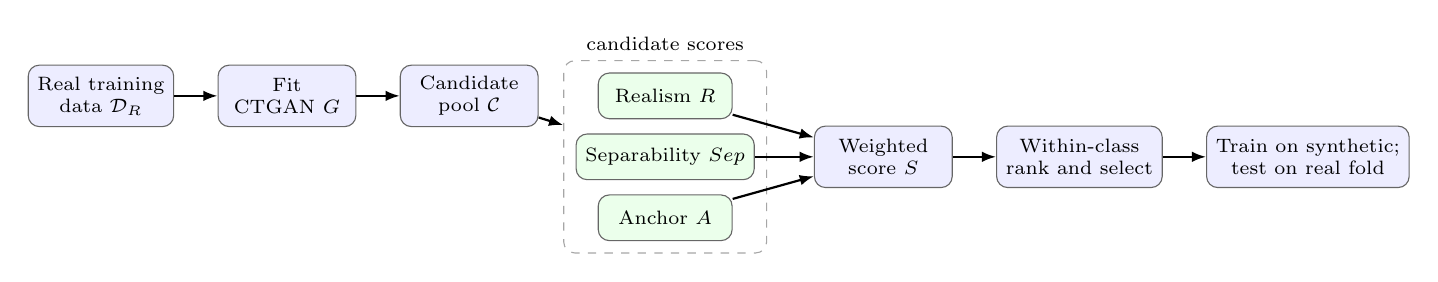
\begin{tikzpicture}[
    node distance=0.55cm,
    block/.style={rectangle, rounded corners, draw=black!60, fill=blue!7,
        minimum width=1.75cm, minimum height=0.78cm, align=center, font=\scriptsize},
    score/.style={rectangle, rounded corners, draw=black!60, fill=green!8,
        minimum width=1.70cm, minimum height=0.58cm, align=center, font=\scriptsize},
    arrow/.style={-{Latex[length=1.8mm]}, thick},
    group/.style={rectangle, rounded corners, draw=black!35, dashed, inner sep=0.15cm}
]
\node[block] (real) {Real training\\data $\mathcal{D}_R$};
\node[block, right=of real] (ctgan) {Fit\\CTGAN $G$};
\node[block, right=of ctgan] (pool) {Candidate\\pool $\mathcal{C}$};

\node[score, right=0.75cm of pool] (realism) {Realism $R$};
\node[score, below=0.18cm of realism] (sep) {Separability $Sep$};
\node[score, below=0.18cm of sep] (anchor) {Anchor $A$};
\node[group, fit=(realism)(sep)(anchor), label={[font=\scriptsize]above:candidate scores}] (scores) {};

\node[block, right=0.75cm of sep] (final) {Weighted\\score $S$};
\node[block, right=of final] (select) {Within-class\\rank and select};
\node[block, right=of select] (eval) {Train on synthetic;\\test on real fold};

\draw[arrow] (real) -- (ctgan);
\draw[arrow] (ctgan) -- (pool);
\draw[arrow] (pool) -- (scores);
\draw[arrow] (realism) -- (final);
\draw[arrow] (sep) -- (final);
\draw[arrow] (anchor) -- (final);
\draw[arrow] (final) -- (select);
\draw[arrow] (select) -- (eval);
\end{tikzpicture}%
}
\caption{SepAware post-generation selection pipeline. Every operation is fitted or computed using the real training portion of a cross-validation fold; the held-out real fold is used only for evaluation.}
\label{fig:sepaware_pipeline}
\end{figure}

The design guards against one simple alternative explanation: SepAware preserves the real class counts, so its TSTR change cannot be caused by a different class ratio. It does not yet eliminate harder alternatives. Ranking can select unusually easy prototypes, discard boundary cases, or amplify a classifier-specific shortcut. These possibilities determine the confirmatory analyses in Chapter~\ref{chap:future}.

\section{Fidelity, separability, and privacy proxies}

Fidelity combines numerical-distribution similarity, categorical-proportion similarity, and correlation preservation. Separability is reported using cosine silhouette, a one-nearest-neighbour label-agreement index (SI), and hypothesis margin (HM). These are descriptive geometric measures; higher separation is not automatically clinically desirable.

Repository privacy analyses include exact-overlap and nearest-neighbour checks in SepAware. They are privacy diagnostics, not formal guarantees. A convincing release claim requires membership- and attribute-inference attacks and, where appropriate, a stated differential-privacy budget.

\section{Replicated $2^2$ factorial experiment}

Let $A\in\{-1,+1\}$ encode separability pressure and $B\in\{-1,+1\}$ anchor pressure. The fold-level response is the classifier-averaged TSTR Macro-F1:
\begin{equation}
y_{ijk}=\mu+q_A A_i+q_B B_j+q_{AB}A_iB_j+\gamma_k+\varepsilon_{ijk},
\label{eq:blocked}
\end{equation}
where $\gamma_k$ is a fixed fold block. The high-minus-low factorial effects are $2q_A$, $2q_B$, and $2q_{AB}$. Type-II ANOVA partitions sums of squares among factors, interaction, fold, and residual error. The primary variation percentages exclude the fold block from the denominator so that factor contributions are compared with experimental error. A slide-style unblocked $2^2r$ calculation is retained in the audit outputs, but Equation~\ref{eq:blocked} is more defensible for paired CV conditions.

Raw and log responses are analysed. Residual normality is assessed using Q--Q plots, Shapiro--Wilk and Jarque--Bera tests. Constant variance is assessed with median-centred Levene (Brown--Forsythe), Fligner--Killeen, and Breusch--Pagan tests. Durbin--Watson and lag-one Ljung--Box tests diagnose ordering-related serial patterns, but cannot establish independence. Different five-fold training sets overlap by 75\%, and conditions within a fold are paired; inference is therefore exploratory.

\section{Domain-anchored causal plausibility filtering}

DACPF generates minority-class CTGAN candidates and ranks their consistency with real minority distributions for domain anchors. The completed COVID experiment compares no augmentation, standard CTGAN augmentation, age filtering, disease-anchor filtering, and combined filtering. This is not causal discovery and does not estimate interventions. ``Causal'' refers to the origin of the anchor hypotheses; the empirical operation is a plausibility filter.

\section{Reproducibility and result authority}

For duplicated studies, executed five-fold notebooks and exported CSV tables take precedence over slide notes, single-split ablations, and earlier drafts. The fixed-lambda authority is the newly executed combined five-fold notebook and its fold-level CSVs. The factorial values are the 40 observations exported to \path{results/actual_2k_r_macro_f1_raw_and_log.csv}. The completed DACPF authority is its five-fold raw-results CSV plus its summary CSV. Generated manuscript figures are reproducible through \texttt{generate\_figures.py}.

\chapter{Empirical Development of Separability-Aware Synthesis}
\label{chap:completed}

\section{From class rebalancing to a separability hypothesis}

The research began from the conventional explanation for poor rare-outcome prediction: the minority class supplies too few examples. Repository experiments consequently examined ordinary rebalancing, CTGAN minority augmentation, and increasingly targeted candidate filters. Their common result was not that augmentation never helped, but that additional minority records did not produce a sufficiently large and consistent gain to explain the problem by class frequency alone. Some early notebooks were single-split or diagnostic studies and are therefore retained as hypothesis-generating evidence rather than reported as confirmatory estimates.

The leakage-controlled DACPF rerun provides the strongest five-fold evidence from this stage (Table~\ref{tab:dacpf}). Standard CTGAN augmentation improves mean Macro-F1 relative to real-only training for both locally available classifiers. Adding an age filter or a combined age-and-disease filter does not improve on standard CTGAN. Disease-anchor filtering performs best, adding 0.0508 over standard CTGAN for CatBoost but only 0.0084 for XGBoost. Thus domain targeting can help, but the effect depends on the anchor and classifier; adding more constraints is not monotonically beneficial.

\begin{table}[htbp]
\centering
\caption{Five-fold COVID-19 augmentation Macro-F1. These are Real+Synthetic$\rightarrow$Real results and are not directly comparable with the standalone-synthetic TSTR studies below.}
\label{tab:dacpf}
\begin{tabular}{lrr}
\toprule
Condition & CatBoost & XGBoost\\
\midrule
Real only & 0.4740 & 0.4759\\
Real + standard CTGAN & 0.5262 & 0.5255\\
Real + age-filtered CTGAN & 0.5257 & 0.4983\\
Real + disease-filtered CTGAN & \textbf{0.5771} & \textbf{0.5339}\\
Real + combined DACPF & 0.5256 & 0.5204\\
\bottomrule
\end{tabular}
\end{table}

\begin{figure}[htbp]
\centering
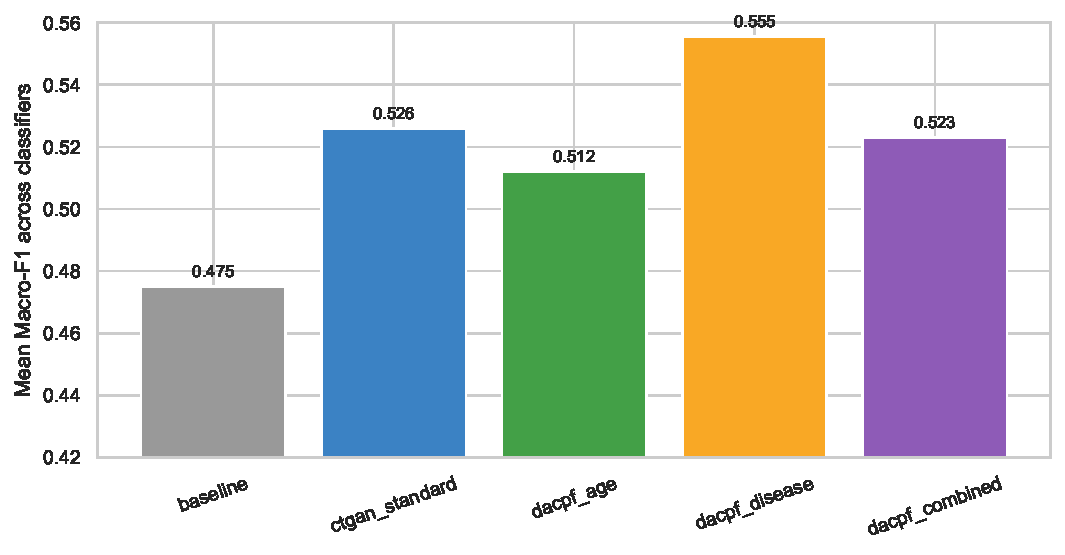
\includegraphics[width=.75\textwidth]{covid_dacpf_summary.pdf}
\caption{COVID-19 DACPF Macro-F1 averaged across CatBoost and XGBoost. The classifier-specific values in Table~\ref{tab:dacpf} show why the average should not be interpreted as a universal anchor effect.}
\label{fig:dacpf}
\end{figure}

This stage ruled out a simple monotonic story in which balancing, generating more cases, or imposing more domain constraints necessarily improves prediction. Explainability and neighbourhood notebooks were then used to examine diversity, class-wise recall, feature-importance shifts, silhouette, nearest-neighbour label agreement, and hypothesis margin. Because some of these analyses used representative folds or earlier configurations, they establish the diagnostic rationale rather than a new numerical result. Their scientific implication was that weak or unstable class geometry remained after augmentation. That observation led to the working hypothesis that class overlap, rather than imbalance alone, was limiting synthetic-to-real transfer.

\section{Testing separability as an explicit generation objective}

SepAware is the intervention implied by that diagnosis. It does not change the target class counts; it asks whether records selected for label-consistent geometry transfer better to held-out real cases. The fixed-lambda experiment fits the complete pipeline independently in five stratified folds. Table~\ref{tab:fixedutility} reports classifier-averaged fold means and 95\% $t$ intervals. On COVID-19, the balanced setting reaches 0.5492 Macro-F1, but its interval is wide. On Vigitel, both the varied grid and fixed high-separability setting reach approximately 0.58 and outperform ordinary CTGAN in all ten matched fold--classifier comparisons. The varied-grid result remains exploratory because configuration selection and performance reporting use the same folds.

\begin{table}[htbp]
\centering
\caption{Corrected five-fold TSTR Macro-F1. Means and 95\% intervals are computed from five classifier-averaged fold scores.}
\label{tab:fixedutility}
\begin{tabular}{llrr}
\toprule
Dataset & Training data & Mean & 95\% half-width\\
\midrule
\multirow{4}{*}{COVID} & Real & 0.5069 & 0.0690\\
& Standard CTGAN & 0.4627 & 0.0407\\
& SepAware varied grid & 0.5350 & 0.0649\\
& Fixed balanced $(1.0,0.5)$ & \textbf{0.5492} & 0.0959\\
\midrule
\multirow{4}{*}{Vigitel} & Real & 0.4672 & 0.0088\\
& Standard CTGAN & 0.4588 & 0.0107\\
& SepAware varied grid & \textbf{0.5839} & 0.0225\\
& Fixed balanced $(1.0,0.5)$ & 0.5834 & 0.0216\\
\bottomrule
\end{tabular}
\end{table}

\begin{figure}[htbp]
\centering
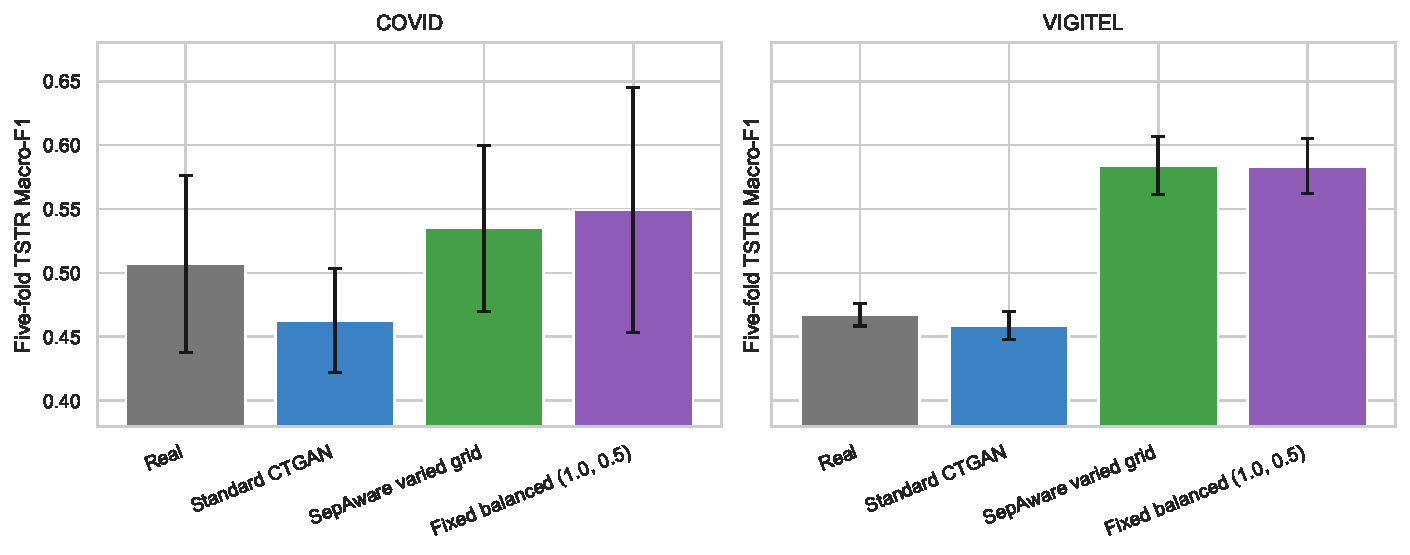
\includegraphics[width=.9\textwidth]{fixed_lambda_fivefold_utility.pdf}
\caption{Corrected five-fold TSTR Macro-F1 for the principal fixed-lambda comparison. Error bars are 95\% $t$ intervals over the five classifier-averaged fold scores.}
\label{fig:fixedutility}
\end{figure}

Table~\ref{tab:lambda} reports the highest mean selection scores from the same run. The repository composite quality varies little, whereas SI and HM respond strongly to separability pressure. Figure~\ref{fig:lambda-tradeoff} makes the same point over the grid: global fidelity is comparatively stable while separability changes. This is evidence that the selector controls a property not captured by the composite quality score. It is not evidence that the selected records are clinically representative.

\begin{table}[htbp]
\centering
\caption{Top executed SepAware grid configurations. ``Quality'' is the repository composite score.}
\label{tab:lambda}
\resizebox{\textwidth}{!}{%
\begin{tabular}{llrrrr}
\toprule
Dataset & $(\lambda_{sep},\lambda_{anchor})$ & Quality & SI & HM & Selection\\
\midrule
COVID & $(1.0,0.0)$ & 0.956 & 0.779 & 0.897 & 2.154\\
COVID & $(1.0,0.25)$ & 0.961 & 0.760 & 0.854 & 2.095\\
COVID & $(1.0,0.5)$ & 0.965 & 0.754 & 0.830 & 2.067\\
Vigitel & $(1.0,0.5)$ & 0.967 & 0.812 & 0.829 & 2.124\\
Vigitel & $(1.0,0.25)$ & 0.967 & 0.811 & 0.822 & 2.116\\
Vigitel & $(1.0,0.0)$ & 0.966 & 0.811 & 0.822 & 2.116\\
\bottomrule
\end{tabular}
}
\end{table}

\begin{figure}[htbp]
\centering
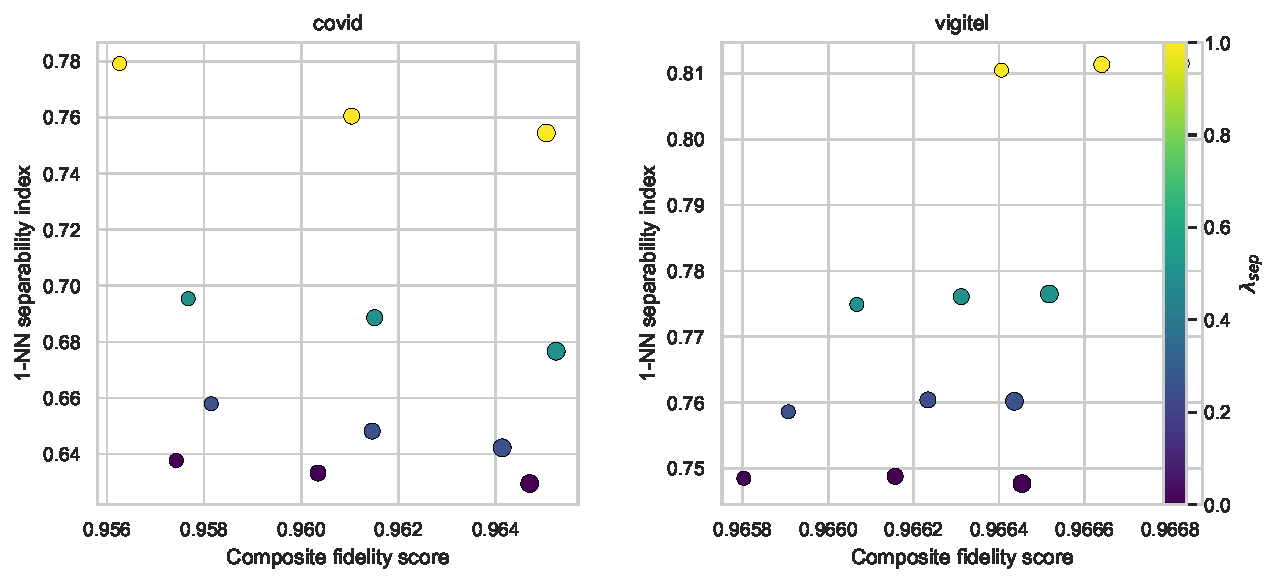
\includegraphics[width=.88\textwidth]{lambda_fidelity_separability.pdf}
\caption{Five-fold mean fidelity--separability trade-off across executed lambda settings. Colour represents separability weight; larger markers represent stronger anchor weight.}
\label{fig:lambda-tradeoff}
\end{figure}

\section{Attributing the gain: replicated factorial experiment}

The fixed-lambda results raised a sharper causal question about the algorithm: was the apparent gain produced by separability pressure, anchor pressure, or their interaction? The replicated $2^2$ experiment answers this component-level question under four predeclared settings. Figure~\ref{fig:foldprofiles} displays all 40 fold responses. COVID-19 profiles cross and exhibit substantial fold variation; Vigitel exhibits a stable step when separability is enabled.

\begin{figure}[htbp]
\centering
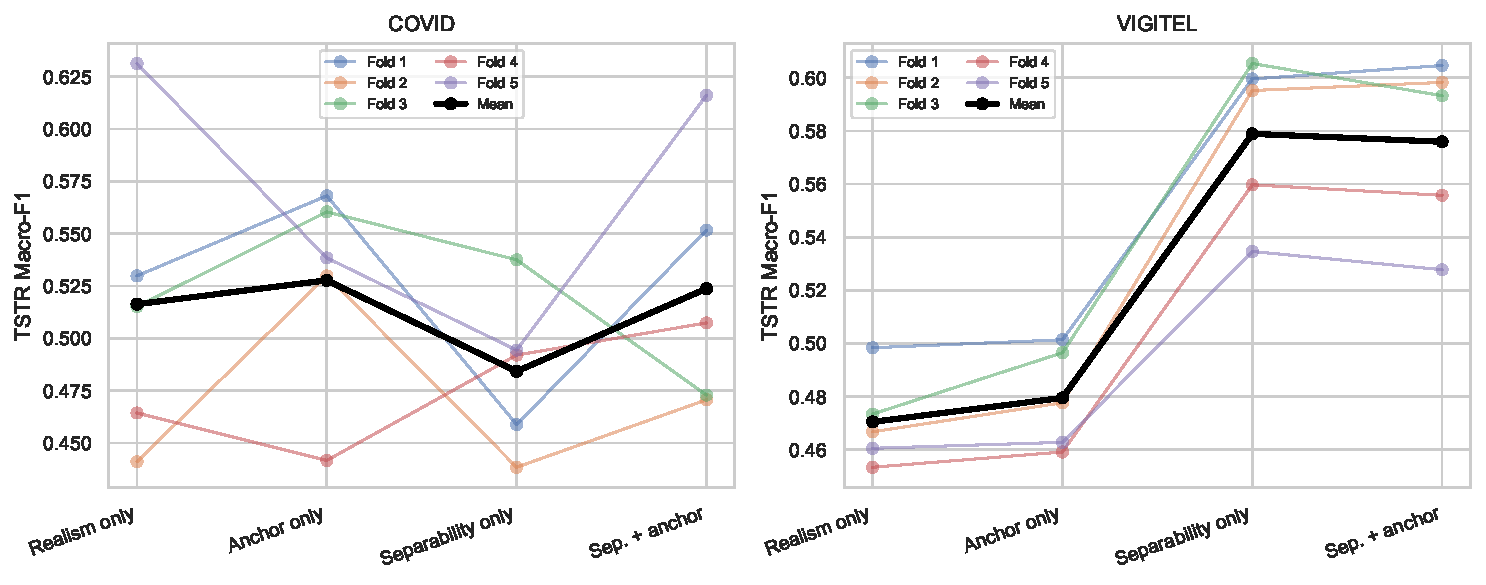
\includegraphics[width=.95\textwidth]{factorial_fold_profiles.pdf}
\caption{Fold-level TSTR Macro-F1 in the replicated $2^2$ SepAware experiment. Black lines show condition means.}
\label{fig:foldprofiles}
\end{figure}

\begin{table}[htbp]
\centering
\caption{Mean TSTR Macro-F1 by predeclared factorial condition. Values are means of the five exported fold responses.}
\label{tab:conditionmeans}
\begin{tabular}{lrrrr}
\toprule
Dataset & Realism only & Anchor only & Separability only & Both\\
\midrule
COVID & 0.516 & 0.528 & 0.484 & 0.524\\
Vigitel & 0.470 & 0.480 & 0.579 & 0.576\\
\bottomrule
\end{tabular}
\end{table}

The condition means in Table~\ref{tab:conditionmeans} show the contrast directly. In Vigitel, enabling separability increases the mean from approximately 0.47--0.48 to 0.576--0.579, whereas adding anchors makes little difference. COVID-19 shows no corresponding ordering: separability-only is the lowest condition mean and the ``both'' condition approximately returns to realism-only performance.

The blocked raw-scale ANOVA in Table~\ref{tab:anova} is the primary component analysis. For COVID-19, none of the treatment effects is significant and residual error accounts for 81.53\% of treatment-plus-error variation after separating the fold block. For Vigitel, separability accounts for 96.00\% and is highly significant; anchor and interaction contributions are negligible. The log-scale model gives the same scientific conclusion. The experiment therefore supports H2 for Vigitel, rejects a dataset-independent version of H2, and supports H3.

\begin{table}[htbp]
\centering
\caption{Blocked factorial ANOVA: percentage of experimental variation and $p$-values on raw Macro-F1. Percentages exclude fold SS from the denominator.}
\label{tab:anova}
\begin{tabular}{llrr}
\toprule
Dataset & Source & Variation (\%) & $p$\\
\midrule
\multirow{4}{*}{COVID} & Separability & 5.13 & 0.4019\\
& Anchor & 10.21 & 0.2439\\
& Interaction & 3.13 & 0.5103\\
& Error & 81.53 & \NA\\
\midrule
\multirow{4}{*}{Vigitel} & Separability & 96.00 & $5.03\times10^{-10}$\\
& Anchor & 0.08 & 0.6069\\
& Interaction & 0.33 & 0.3154\\
& Error & 3.59 & \NA\\
\bottomrule
\end{tabular}
\end{table}

\begin{figure}[htbp]
\centering
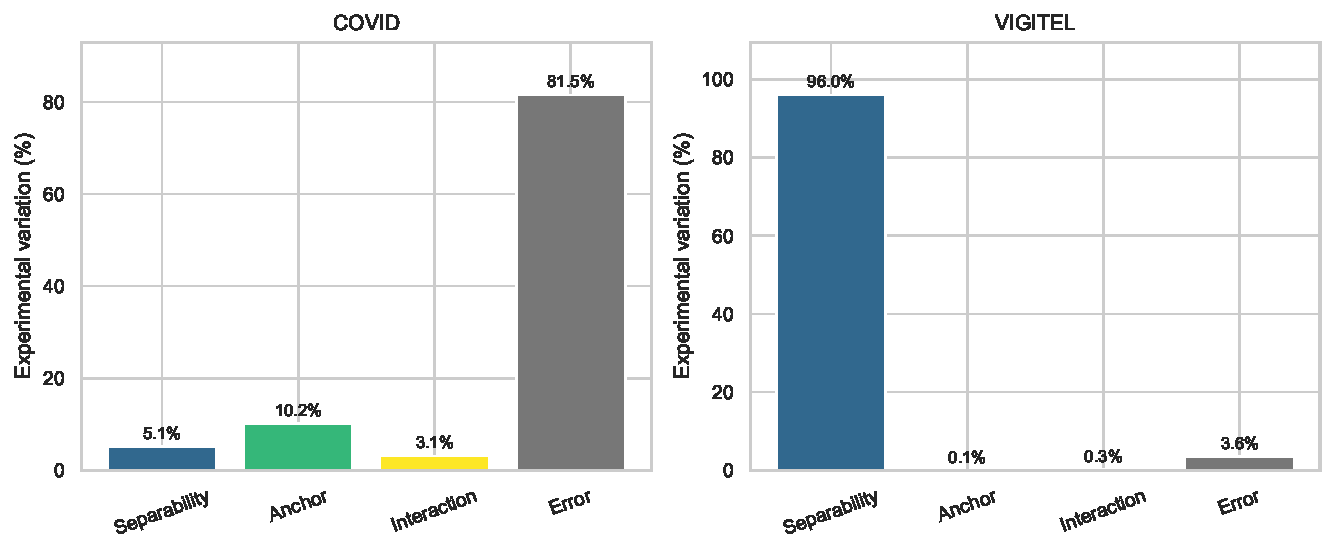
\includegraphics[width=.88\textwidth]{factorial_variation.pdf}
\caption{Variation allocation for the blocked raw-scale factorial models.}
\label{fig:variation}
\end{figure}

\begin{table}[htbp]
\centering
\caption{Residual assumption diagnostics for the blocked factorial models.}
\label{tab:assumptions}
\resizebox{\textwidth}{!}{%
\begin{tabular}{llrrrrp{2.5cm}}
\toprule
Dataset & Scale & Shapiro & B--F & Fligner & B--P & Assessment\\
\midrule
COVID & raw & .2446 & .8409 & .8394 & .4415 & no detected violation\\
COVID & log & .2031 & .8173 & .8050 & .6435 & no detected violation\\
Vigitel & raw & .8564 & .8413 & .7706 & .0186 & variance flag\\
Vigitel & log & .8625 & .7463 & .6834 & .0237 & variance flag\\
\bottomrule
\end{tabular}
}
\end{table}

Normality tests do not reject for either dataset. Vigitel's groupwise robust tests do not reject equal variance, but Breusch--Pagan does; the log transform does not resolve the conflict. More importantly, independence is not established because cross-validation training sets overlap and the four conditions within each fold share a candidate pool. The very small Vigitel residual should therefore be tested across independent generator and partition seeds before it is treated as a stable population effect.

\section{What the completed evidence establishes}

The experiments form a coherent progression. Rebalancing and unconstrained augmentation did not make utility reliably high; domain filters sometimes helped but did not behave monotonically; diagnostic analyses implicated class overlap; SepAware then improved Vigitel TSTR while measured composite fidelity remained broadly stable; and the factorial study attributed that gain to separability rather than anchors. The COVID-19 null result is equally informative: explicit separability is not sufficient when the positive class is small, heterogeneous, or weakly represented.

The evidence does not yet show that SepAware recovers clinically meaningful signal. An alternative explanation is that it deletes ambiguous observations and manufactures an easier classification problem. Nor does the current factorial design establish generalisation beyond CTGAN, these datasets, these classifiers, or the recorded seeds. These are not peripheral limitations; they define the tests required to turn the present method into a contribution to knowledge.

\chapter{Interpretation, Rival Explanations, and Validity}
\label{chap:discussion}

\section{Interpretation of the proposed mechanism}

Across the SepAware lambda grid, composite fidelity changes only modestly while SI and HM change substantially. In the factorial study, enabling separability increases Vigitel Macro-F1 by approximately 0.10, while anchor pressure contributes essentially nothing. The strongest empirically supported contribution is therefore not a universally optimal generator. It is evidence, in one dataset, that a transparent post-generation objective controls a utility-relevant dimension that the current global fidelity score obscures. The factorial result strengthens this interpretation because the Vigitel change follows the separability factor and not the anchor factor.

The COVID-19 results constrain that claim. The fixed-lambda study suggests a possible average improvement, but its interval is wide; in the predeclared factorial analysis, treatment effects are small relative to fold variation and are not significant. A scalar margin may be ineffective when minority mortality cases are heterogeneous, or may select easy but unrepresentative prototypes. Stronger separation can mean clearer signal, but it can also mean removal of difficult patients, comorbidity interactions, or label ambiguity.

\section{Alternative explanation: an artificially easier problem}

The principal challenge to SepAware is also the most important scientific question for the thesis. Higher TSTR performance may arise because selection recovers class-conditional signal that CTGAN generated but did not concentrate. It may instead arise because selection removes borderline observations, narrows minority modes, or amplifies a relationship peculiar to the training fold. Held-out-real testing prevents a wholly synthetic self-consistency result, but does not distinguish these mechanisms. Boundary-stratified errors, calibration, real-minority cluster retention, label-permutation controls, and suspected-shortcut masking are required. If gains occur only for easy cases or disappear after shortcut control, the contribution must be narrowed.

\section{Minority preservation and clinical realism}

Preserving prevalence is necessary but insufficient. A synthetic dataset can reproduce 83 deaths while collapsing distinct death phenotypes into one mode. SI and HM detect geometric cohesion but cannot determine whether clinically important subgroups survive. Evaluation must therefore include class-conditional distributions and dependencies, minority precision and recall, AUPRC, subgroup coverage, calibration, and within-positive-class diversity.

The DACPF results reinforce this interpretation. Disease filtering improves both available classifiers relative to standard CTGAN, whereas age-only and combined filtering do not. Anchors may be redundant, misdirected, or too aggressively weighted. Domain knowledge should constrain implausibility without forcing every patient towards a class centroid. Blinded clinician review of cases and cohort relationships is needed because geometric scores cannot detect every incoherent clinical combination.

\section{Does causal information add value?}

The present experiments do not identify causal effects. Anchor--target associations can reflect confounding, selection, measurement, or coding. A DAG learned from 334 COVID-19 records would also be unstable without priors and bootstrap analysis. Moreover, DACPF does not demonstrate value from causal knowledge as such: disease anchors help in some comparisons, age and combined filters do not, and no association-matched non-causal control was included. The defensible interpretation is narrower. Causal hypotheses can supply auditable constraints and diagnostics; their incremental value must be isolated against matched associational controls and graph uncertainty.

\section{Privacy implications}

Nearest-neighbour distances and absence of exact duplicates are sanity checks, not evidence of anonymity. SepAware prefers candidates close to the real manifold, which may improve utility and increase disclosure risk. Membership and attribute inference, nearest-record distributions stratified by rarity, and differentially private variants are therefore required before a release claim. Privacy is an optimisation axis, not an assumed consequence of synthesis.

\section{Statistical limitations}

Five-fold cross-validation supplies five performance estimates, but the training sets overlap. Within-fold factorial conditions also share a generator and candidate pool. Blocking by fold is appropriate for paired contrasts, yet conventional ANOVA $p$-values remain approximate. Repeated nested cross-validation across independent partition and generator seeds is required for confirmatory inference. Vigitel's Breusch--Pagan result further supports robust or bootstrap intervals.

The factorial endpoint averages CatBoost and XGBoost within fold. This simplifies attribution but can mask a treatment-by-classifier interaction. A confirmatory model should retain classifier as a repeated factor and report prespecified classifier-specific contrasts. The Vigitel $p$-value is conditional on this experimental design; it is not the probability that SepAware will succeed on a new dataset.

\section{Threats to validity}

\paragraph{Internal validity.} Several notebooks evolved across protocol revisions, and exploratory lambda selection can reuse information later reported as performance. The evidence audit identifies the authoritative reruns but cannot retroactively create preregistration.

\paragraph{Construct validity.} Composite quality, SI, HM, and anchor scores are engineering proxies. They do not directly measure clinical realism, causal validity, patient benefit, or minority-mode coverage.

\paragraph{External validity.} The strongest factorial effect occurs in one Vigitel sample; COVID-19 contains only 334 records. SepAware has not been tested across sites, periods, outcomes, generators, or substantially different imbalance ratios.

\paragraph{Conclusion validity.} One cross-validation partition and limited generator seeds do not quantify synthesis stochasticity. Multiple metrics and configurations increase researcher degrees of freedom unless endpoints and comparisons are prespecified.

\paragraph{Privacy validity.} Empirical similarity diagnostics are not a formal guarantee and do not simulate an adversary with auxiliary clinical information.

\section[Defence questions]{Questions expected at qualification defence}

\begin{description}[leftmargin=*,style=nextline]
\item[Is SepAware merely making classification easier?]
Possibly. Held-out-real evaluation is necessary but insufficient. Boundary-stratified errors, calibration, mode coverage, shortcut controls, and external validation are the decisive tests.

\item[Why separability rather than imbalance?]
The claim is comparative, not exclusive. SepAware preserves class counts across factorial conditions, yet Vigitel utility changes sharply with separability pressure. This isolates a within-experiment separability effect; a controlled imbalance-by-overlap study is still needed for generalisation.

\item[Are the gains robust?]
Not yet at thesis level. Vigitel is consistent across the recorded folds, whereas COVID-19 is not. Independent partition, synthesis, and classifier seeds are required.

\item[Does SepAware generalise?]
No such claim is currently supported. CTGAN is the common candidate generator and the strong effect occurs in one survey dataset. Diffusion, VAE, copula, and strong resampling baselines plus external clinical datasets are necessary.

\item[Does stable global fidelity rule out unrealistic data?]
No. It shows only that the measured aggregate score changed little. It may hide minority collapse, implausible multivariate combinations, and calibration loss.

\item[What does the causal component contribute?]
At present it supplies domain-motivated hypotheses and a negative result about hard filtering, not causal validity. Its incremental value must be tested against association-matched controls.

\item[Does selection affect privacy?]
It may increase risk by preferring candidates near real records, especially rare ones. Attack-based and differential-privacy evaluation are essential.
\end{description}

\section{Present answer to the research questions}

The first question is answered provisionally: augmentation alone does not resolve weak class geometry, although it can yield modest or classifier-dependent improvements. The second is answered conditionally: separability-aware selection is strongly effective for Vigitel but not demonstrated for COVID-19. The factorial experiment answers the third for Vigitel by attributing the gain to separability rather than anchors; it provides no corresponding COVID-19 attribution. The fourth remains open because clinical realism, minority coverage, shortcut behaviour, privacy, and external transfer have not yet been tested sufficiently. Chapter~\ref{chap:future} is designed to resolve that question rather than append unrelated models.

\chapter{Research Programme to Establish Generality and Clinical Validity}
\label{chap:future}

The remaining PhD is organised as four connected studies. Each addresses a rival explanation raised by the completed work, and each supplies evidence needed by the next. The programme moves from mechanism identification, through confirmatory benchmarking and safety evaluation, to a new constrained generator and external validation.

\section{Study 1: Separate imbalance from intrinsic class overlap}

\textbf{Research question.} Is the benefit of SepAware caused by class imbalance, class overlap, or their interaction?

\textbf{Hypothesis.} Changing prevalence will affect classifier variance and threshold behaviour, but SepAware will add utility principally when recoverable class-conditional signal exists in an overlapping minority distribution.

\textbf{Method.} Construct controlled semi-synthetic benchmarks from the real feature spaces in which prevalence and Bayes overlap vary independently. On real datasets, create prespecified training prevalences by training-fold subsampling while leaving the real test distribution unchanged. Compare no resampling, random over- and undersampling, SMOTE, class weighting, standard CTGAN, and SepAware under identical folds and sample budgets.

\textbf{Evaluation.} Estimate Macro-F1, minority F1, AUPRC, calibration, boundary-stratified error, and sample efficiency over repeated partition and model seeds. Fit a hierarchical interaction model for imbalance, overlap, method, classifier, and dataset.

\textbf{Expected contribution.} This study will identify when separability is a genuine missing objective rather than a proxy for class rebalancing.

\section{Study 2: Confirm utility without minority-mode collapse}

\textbf{Research question.} Does separability-aware selection improve held-out-real minority performance across datasets, generators, classifiers, and random seeds without deleting difficult but valid cases?

\textbf{Hypothesis.} Moderate class-conditional pressure will improve Macro-F1 and AUPRC when the minority distribution is learnable, whereas aggressive pressure will reduce boundary coverage, calibration, or within-class diversity.

\textbf{Method.} Predeclare lambda values and endpoints; use nested five-fold cross-validation across at least ten partition seeds and independent generator seeds. Compare CTGAN, TVAE, a Gaussian-copula baseline, TabDDPM, random resampling, SMOTE, and class weighting. Apply the selector to more than one candidate generator to test whether it is generator agnostic. Evaluate TSTR and augmentation separately. Add diversity quotas or cluster coverage so that one minority phenotype cannot dominate selection.

\textbf{Evaluation.} Report Macro-F1, minority precision/recall/F1, AUROC, AUPRC, calibration, decision-curve utility, class-conditional fidelity, coverage, discriminator AUC, and seed-level uncertainty. Analyse errors by distance to the real training boundary and by minority cluster. Use paired hierarchical bootstrap or mixed-effects models retaining dataset, partition, fold, generator seed, generator, and classifier.

\textbf{Expected contribution.} This study will establish the reproducibility envelope and failure modes of separability-aware selection, including whether its gains reflect shortcut amplification or loss of ambiguous patients.

\section{Study 3: Test causal, clinical, and privacy consistency}

\textbf{Research question.} Can synthetic selection preserve a credible range of causal relations and clinical phenotypes without increasing disclosure risk?

\textbf{Hypothesis.} Fidelity- or separability-only selection will preserve some pairwise associations but violate stable conditional independences, clinically reviewed constraints, or privacy thresholds; soft uncertainty-aware constraints will outperform hard anchor filters.

\textbf{Method.} Construct a partially directed expert graph for each dataset, documenting required, forbidden, and uncertain edges. Bootstrap NOTEARS and constraint-based discovery on real training data to quantify edge stability. Compare causal anchors with association-matched control anchors. Define structural and conditional-independence discrepancies, and use semi-synthetic structural causal models where intervention ground truth is available.

\textbf{Evaluation.} Compare synthetic-to-real graph discrepancy with real bootstrap variability. Include permuted-label and DAG-violating negative controls. Clinicians will conduct blinded case-level plausibility and cohort-relationship review. Membership inference, attribute inference, exact/near duplication, and rarity-stratified nearest-neighbour risk will assess disclosure; differentially private variants will provide privacy-budget comparisons.

\textbf{Expected contribution.} The result will be an uncertainty-aware evaluation framework that separates clinical plausibility, causal consistency, and privacy from geometric separability.

\section{Study 4: Causally constrained generation and external validation}

\textbf{Research question.} Can a graph-informed generator improve rare-outcome utility and causal consistency across datasets and distribution shifts without sacrificing diversity or privacy?

\textbf{Hypothesis.} A latent tabular diffusion model with soft structural penalties, class-conditional guidance, and diversity regularisation will outperform hard row filtering, but its advantage will narrow under external shift and stronger privacy constraints.

\textbf{Method.} Extend tabular diffusion with conditional rare-outcome generation, differentiable penalties for stable graph constraints, distributional rather than pointwise anchors, and minority-diversity regularisation. Compare it with CTGAN+SepAware, TVAE, unconstrained diffusion, DACPF, and Study~1 imbalance baselines. Train on one Vigitel period or clinical source and test on another; include at least one external health dataset with a distinct outcome and imbalance ratio.

\textbf{Evaluation.} Use the full Study~2 utility panel and Study~3 causal, clinical, and privacy metrics, with ablations for every constraint. Produce Pareto fronts across fidelity, utility, causal consistency, subgroup disparity, and attack success. Semi-synthetic data will support causal-truth claims; observational data will support only plausibility and transfer claims.

\textbf{Expected contribution.} This study provides the thesis's central methodological and external-validity test: whether utility-aware, uncertainty-constrained synthesis generalises beyond the dataset and generator from which SepAware emerged.

\section{Decision criteria and thesis-level contribution}

SepAware will be considered supported only if its utility advantage persists across prespecified seeds and classifiers, does not materially degrade class-conditional coverage or calibration, survives shortcut controls, and transfers to external real data. Causal constraints will be retained only if they improve consistency beyond association-matched controls. Privacy conclusions will be limited to the stated threat model and, where used, differential-privacy budget.

If these criteria are met, the contribution to knowledge will comprise: (i) evidence that separability is a controllable determinant of synthetic-to-real utility distinct from class prevalence and aggregate fidelity; (ii) a validated selection framework that balances utility with minority diversity and realism; (iii) an uncertainty-aware causal and clinical evaluation framework; and (iv) a causally constrained generative method evaluated under external shift and explicit privacy risk. If some criteria fail, the negative boundary conditions will remain a substantive contribution by showing when separability optimisation should not be used.

\section{Publication pathway}

The nearest publication is a rigorous cross-dataset evaluation of transparent selection guided by class separability. Its novelty is not a new GAN architecture, but controlled evidence that class-boundary preservation is independently tunable, together with factorial attribution and a clinically important failure analysis. Before submission, Study~1 and the confirmatory portion of Study~2 are essential, as are class-conditional fidelity, minority/AUPRC metrics, privacy attacks, and at least one external validation. The separate CBM readiness note records the proposed title, current support, missing experiments, and likely reviewer concerns.

\chapter{Conclusion}
\label{chap:conclusion}

\begin{sloppypar}
This qualification develops one scientific argument. Rebalancing and unconstrained augmentation do not necessarily resolve weak prediction when outcome classes overlap. Domain-guided filtering can help, but its effects depend on the anchor and classifier. This motivated a separability diagnosis and then SepAware, an explicit intervention on class-conditional geometry. The factorial experiment attributes the strong Vigitel TSTR gain to separability pressure: it explains 96.00\% of treatment-plus-error variation, whereas anchor and interaction contributions are negligible. The corresponding COVID-19 effect is not established; separability explains 5.13\% and residual error 81.53\%.

The current contribution is consequently a method, a component-level empirical finding, and a set of boundary conditions---not proof of universal superiority. SepAware may still select easy prototypes, reduce minority diversity, amplify shortcuts, or increase privacy risk. The remaining programme tests those explanations by separating imbalance from overlap, repeating comparisons across generators and seeds, measuring clinical, causal, and privacy consistency, and validating under external shift. The intended PhD contribution is a defensible account of when separability should be controlled, how it trades against fidelity and safety, and when it should not be used.
\end{sloppypar}


\renewcommand\bibname{References}
\bibliographystyle{plainnat}
\bibliography{referencias}

\begin{apendices}
\chapter{Repository Evidence Audit}
\label{app:audit}

\begin{longtable}{>{\raggedright\arraybackslash}p{.29\textwidth}>{\raggedright\arraybackslash}p{.18\textwidth}>{\raggedright\arraybackslash}p{.45\textwidth}}
\caption{Status of research artefacts used during manuscript reconstruction.}\label{tab:audit}\\
\toprule
Artefact & Status & Manuscript treatment\\
\midrule
\endfirsthead
\toprule
Artefact & Status & Manuscript treatment\\
\midrule
\endhead
Older dataset-specific fixed-lambda notebooks & Superseded single-split studies & Excluded from numerical claims because they use one 75/25 split.\\
Combined SepAware fixed-lambda notebook & Executed five-fold study & Authority for fold-level fixed-lambda comparisons.\\
Protocol-audited $2^2$ CV notebook & Executed & Used for earlier condition summaries and correlation interpretation.\\
Replicated factorial ANOVA notebook with results & Latest executed experiment & Authority for the 40 fold responses, ANOVA, effects, and diagnostics.\\
Factorial assumption-test script/CSVs & Executed after latest notebook & Authority for expanded residual tests and classical-versus-blocked sensitivity analysis.\\
COVID DACPF raw and summary CSVs & Executed & Authority for augmentation results in Table~\ref{tab:dacpf}.\\
TabPFN augmentation notebook & Failed dependency output & Protocol only; no result claim.\\
Unexecuted causal-filter notebooks & Incomplete protocol & Discussed as development history or future work, not evidence.\\
Cluster-then-augment notebook & No authoritative exported result located & Excluded from numerical results.\\
Business analytics notebooks & Out of scientific scope & Excluded.\\
\bottomrule
\end{longtable}

\section{Result-authority decisions}

The newly rerun factorial experiment differs numerically from earlier protocol-audited slide notes because CTGAN is stochastic even under the recorded software stack. This manuscript uses the new executed observations consistently. The classical unblocked Aula~5 decomposition treats folds as replications and assigns COVID 90.01\% error and Vigitel 16.92\% error. The primary manuscript uses the blocked model, which separates fold variation and yields 81.53\% and 3.59\%, respectively. Both calculations exist in the repository; their denominators answer different questions.

No Real+Synthetic results are created for SepAware because its completed factorial protocol evaluates standalone synthetic datasets. Conversely, DACPF is explicitly an augmentation experiment and is labelled Real+Synthetic. Missing AUPRC, calibrated probabilities, formal membership inference, and external validation are not imputed.

\end{apendices}
\end{document}
